% \documentclass[UTF8,12pt,a4paper]{ctexart}
\documentclass[UTF8,12pt,a4paper]{article}

% ------------------------------- 导言区 -----------------------------------
\usepackage{amsmath}
\usepackage{cases}
\usepackage{cite}
\usepackage{graphicx}    % 用于插入图片
\usepackage{subcaption}  % 用于子图布局
\usepackage{enumerate}
\usepackage{algorithm}
\usepackage{caption} %\caption*需要
\usepackage[noend]{algpseudocode} %algorithmicx
\makeatletter
\renewcommand{\fnum@algorithm}{\fname@algorithm}
\makeatother
\renewcommand{\algorithmicrequire}{\textbf{Input:}}
\renewcommand{\algorithmicensure}{\textbf{Output:}}
\usepackage[margin=1in]{geometry}
\geometry{a4paper}
\usepackage{fancyhdr}
\pagestyle{fancy}
\fancyhf{}


% ------------------- 自定义代码展示风格 -----------------
\usepackage{listings}
\usepackage{xcolor}
\lstdefinestyle{hspice}{
    language=C,
    basicstyle=\ttfamily\small,
    keywordstyle=\color{blue}\bfseries,
    commentstyle=\color{green!50!black},
    stringstyle=\color{brown},
    numbers=left,
    numberstyle=\tiny\color{gray},
    stepnumber=1,
    numbersep=5pt,
    backgroundcolor=\color{white},
    showspaces=false,
    showstringspaces=false,
    showtabs=false,
    frame=single,
    rulecolor=\color{black},
    tabsize=2,
    captionpos=b,
    breaklines=true,
    breakatwhitespace=true,
    escapeinside={\%*}{*)},
    morekeywords={param, include, temp, option, probe, DC, dc, measure, alter, VDD, GND, gnd, NMOS, PMOS,FIND, WHEN, sweep, abs, I, SUPPLY, lg, fin_height, fin_width, tran, ac, op, model, end, subckt,ends,global, nmos, pmos},
    comment=[l]{*} % 在这里设置注释
}

\lstset{style=hspice} % 只应用样式

% ------------------- 三线表所需宏包 --------------------
\usepackage{booktabs} % 在导言区添加

% ------------------- 表格与单元格分割  ------------------
\usepackage{multirow}
\usepackage{makecell}
\usepackage{array}
% 让定宽列也能水平居中
\newcolumntype{P}[1]{>{\centering\arraybackslash}p{#1}}
% ------------------- 设置超链接,便于跳转 -----------------
\usepackage{enumitem}
\usepackage{hyperref}
\hypersetup{
    pdfborder={0 0 0},    % 消除超链接边框
    colorlinks=true,       % 将边框改为颜色标记(可选)
    linkcolor=black,       % 内部链接颜色(目录、引用等)
    citecolor=black,       % 引用颜色
    urlcolor=blue          % URL链接颜色(保持蓝色以便区分)
}
% ------------------------------- 标题、autor、目录区 -----------------------------------
\title{DIC Experiment Lab1}
\author{
	Name: \underline{Jun Feng}~~~~~~
	Student ID: \underline{523031910148}~~~~~~}
\date{\today}
\pagenumbering{arabic}

\begin{document}

% 如下两行请按实际情况修改
\fancyhead[L]{Jun Feng}
\fancyhead[C]{DIC Experiment Lab1}
\fancyfoot[C]{\thepage}

\maketitle
\tableofcontents

% ------------------------------- 正文区 -----------------------------------
\newpage
\section{Introduction}
This lab focuses on the simulation and comparison of two key transistor technologies: the planar bulk Silicon MOSFET and the 3D FinFET. As device scaling reaches nanoscale dimensions, the planar MOSFET suffers from poor gate electrostatic control, leading to significant short-channel effects like high leakage current. The FinFET architecture addresses this by employing a vertical "fin" structure, allowing the gate to control the channel from three sides, which dramatically improves performance and reduces leakage.

A critical difference in designing with FinFETs is the concept of width quantization. Unlike planar bulk Silicon MOSFETs, whose width can be arbitrarily sized, the effective width of a FinFET is determined by its physical geometry. The minimum width for a single fin is given by equation \eqref{eq:emin}:
\begin{equation}
	\label{eq:emin}
    W_{\text{min}} = 2 \times H_{\text{fin}} + t_{\text{si}}
\end{equation}

To achieve a larger drive strength of gate, multiple fins are used, making the total effective width given by equation  \eqref{eq:multiple_min}:
\begin{equation}
	\label{eq:multiple_min}
 	W_{\text{total}} = n \times (2 \times H_{\text{fin}} + t_{\text{si}})
\end{equation}

The objective of this lab is to use HSPICE simulations with Predictive Technology Models (PTM) to analyze the DC characteristics of 16nm bulk MOSFETs and 20nm FinFETs. Key tasks include:
\begin{enumerate}
	\item Plot $I_{\text{DS}}-V_{\text{DS}}$ Curves
	\item Measure important parameters: $I_{\text{on}}$, $I_{\text{off}}$ and $V_{\text{T}}$
	\item Optional: Subthrehold Slope(SS)
\end{enumerate}

\newpage
\section{Lab Procedures and Results}

\subsection{Simulation Settings}
\begin{itemize}
	\item $L_{\text{g}} = 20\text{nm}$ for ptm16hp FinFETs while $L_{\text{g}} = 16\text{nm}$ for ptm16hp bulk Si-MOSFETs.
	\item Supply voltage is $0.75\text{V}$ for both FinFETs and bulk SiMOSFETs.
	\item Simulation temperature: $T = 25^\circ$C.
	\item Under 16nm process, $\lambda=8\text{nm}$.
\end{itemize}
\subsection{Task1. Plot $I_{\text{DS}}-V_{\text{DS}}$ Curves}

\subsubsection{Part1. bulk Silicon MOSFETs}
\textbf{Requirements}

For both N-Channel and P-Channel bulk silicon MOSFETs, plot the $I_{\text{DS}}-V_{\text{DS}}$ Curves when the gate-source voltage is fixed at 0.75V. 

At the same time, scanning parameter \textbf{width} increases from $16\lambda$ to $48\lambda$ with a step size of $8\lambda$.

\textbf{Procedures}

\textbf{step1. Parameter Settings and Lib importing}
\begin{lstlisting}
	* parameter config
	.param lambda=8nm
	.param Width='16*lambda'
	.param Vgs_n=0.75
	.param Vgs_p=-0.75
	.temp 25
	* lib config
	.include '../Lab_LIB/Bulk/16nm_HP.pm'
\end{lstlisting}

\textbf{Step2. Stimulus and Device Definition}

Set the NMOS gate voltage to 0.75V, the source and bulk to ground (0V), the channel length to 16nm, and the channel width as the parameter to be scanned, with the value parameter: "Width". Repeat the similar process for the PMOS.
\begin{lstlisting}
	* motivation source for nmos
	VGS_N gate_n 0 'Vgs_n'
	VDS_N drain_n 0 0
	* motivation source for nmos
	VGS_P gate_p 0 'Vgs_p'
	VDS_P drain_p 0 0
	* Bulk device definition for NMOS
	MNFET drain_n gate_n 0 0 nmos L='2*lambda' W='Width'
	* Bulk device definition for PMOS
	MPFET drain_p gate_p 0 0 pmos L='2*lambda' W='Width'
\end{lstlisting}

\textbf{Step3. DC Simulatiojn}

For NMOS, sweep $V_{\text{DS}}$ from 0V to 0.85V, take a point every 0.01V, obtain the drain-source current at each DC operating point, then draw a curve.

Repeat the similar process for the PMOS. It is worth noting that the drain-source $V_{\text{DS}}$ voltage of PMOS needs to be swept from 0V to -0.85V.
\begin{lstlisting}
	* DC analysis - Sweep VDS from 0 to 0.85V for different fin numbers
	.dc VDS_N 0 0.85 0.01 sweep Width '16*lambda' '48*lambda' '8*lambda'
	.probe DC I(VDS_N) 
	.dc VDS_P 0 -0.85 -0.01 sweep Width '16*lambda' '48*lambda' '8*lambda'
	.probe DC I(VDS_P)
\end{lstlisting}

\textbf{Step4. Plot the $I_{\text{DS}}-V_{\text{DS}}$ curve}

From above procedures we obtain two waveform data files: Task1\_Bulk.sw0 and Task\_Bulk.sw1.

In CustomExplorer, we plot the $I_{\text{DS}}-V_{\text{DS}}$ curve for both NMOS(Fig.\ref{fig:NMOS_I_V}) and PMOS(Fig.\ref{fig:PMOS_I_V}). 

It is worth noting that in hspice, the direction of current is defined as positive when flowing into the voltage source and negative when flowing out of the voltage source.

\textbf{Results}

\textbf{1. Widths/lengths of transistors:} Length: 16nm, Width: 128nm, 192nm, 256nm, 320nm, 384nm.

\textbf{2.} $U_{\text{DS}}-V_{\text{DS}}$ \textbf{curves:}
\begin{figure}[htbp]
    \centering
    % 第一张子图
    \begin{subfigure}[b]{0.45\textwidth} % 子图宽度为总宽度的45%
        \centering
        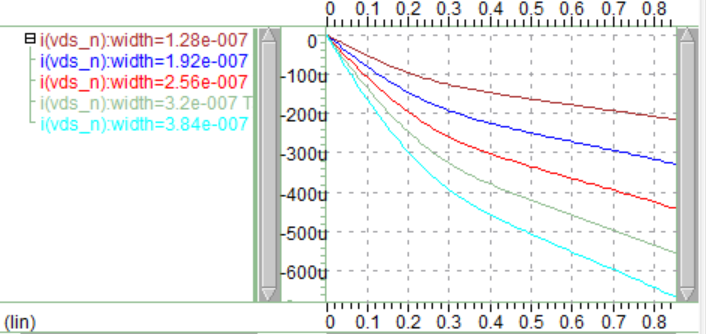
\includegraphics[width=\textwidth]{figure/wv_Task1_Bulk_NMOS_white.png} % 替换为你的图片路径
        \caption{NMOS: $I_{\text{DS}}-V_{\text{DS}}$}
        \label{fig:NMOS_I_V}
    \end{subfigure}
    \hfill % 添加水平间距
    % 第二张子图
    \begin{subfigure}[b]{0.45\textwidth}
        \centering
        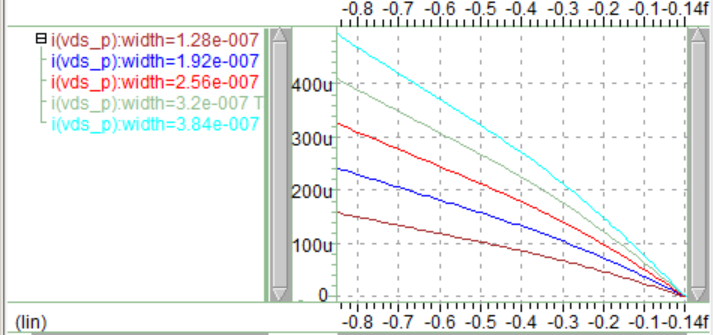
\includegraphics[width=\textwidth]{figure/wv_Task1_Bulk_PMOS_white.png} % 替换为你的图片路径
        \caption{PMOS: $I_{\text{DS}}-V_{\text{DS}}$}
        \label{fig:PMOS_I_V}
    \end{subfigure}
    % 总图标题
    \caption{$I_{\text{DS}}-V_{\text{DS}}$ curve}
    \label{fig:bulk_IV}
\end{figure}


\subsubsection{Part2. FinFETs}

\textbf{Requirements}

For both N-Channel and P-Channel FinFETs, plot the $I_{\text{DS}}-V_{\text{DS}}$ Curves when the gate-source voltage is fixed at 0.75V. 

At the same time, scanning parameter \textbf{fin number} increases from $4$ to $8$ with a step size of $2$.

\textbf{Procedures}

Aside from the parameter sweep during DC simulation, the FinFET simulation steps are identical to those for bulk silicon MOSFETs.
In a FinFET, the effective channel length $L_{g}$ is 20nm, and the channel width is defined by equation \eqref{eq:multiple_min}. A key parameter is the counts of fins. During the FinFET simulation, the counts of fins is swept from 4 to 8 with a step size of 2: 
\begin{lstlisting}
	* DC analysis - Sweep VDS from 0 to 0.85V for different fin numbers
	.dc VDS_N 0 0.85 0.01 sweep Nfin 4 8 2
	.probe DC I(VDS_N) 
	.dc VDS_P 0 -0.85 -0.01 sweep Nfin 4 8 2
	.probe DC I(VDS_P)
\end{lstlisting}

In CustomExplorer, we plot the $I_{\text{DS}}-V_{\text{DS}}$ curve for both NFET(Fig.\ref{fig:NFET_I_V}) and PFET(Fig.\ref{fig:PFET_I_V}). 

\textbf{Results}

\textbf{1. Widths/lengths of transistors:} Length: 20nm, Width: 256, 384nm, 512nm

\textbf{2.} $U_{\text{DS}}-V_{\text{DS}}$ \textbf{curves:}
\begin{figure}[htbp]
    \centering
    % 第一张子图
    \begin{subfigure}[b]{0.45\textwidth} % 子图宽度为总宽度的45%
        \centering
        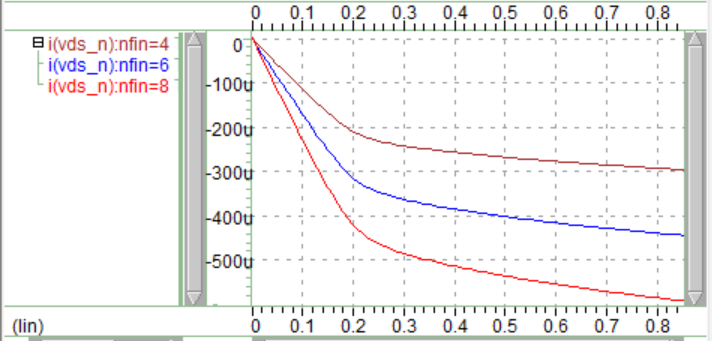
\includegraphics[width=\textwidth]{figure/wv_Task1_Fin_NFET.png} 
        \caption{NMOS: $I_{\text{DS}}-V_{\text{DS}}$}
        \label{fig:NFET_I_V}
    \end{subfigure}
    \hfill % 添加水平间距
    % 第二张子图
    \begin{subfigure}[b]{0.45\textwidth}
        \centering
        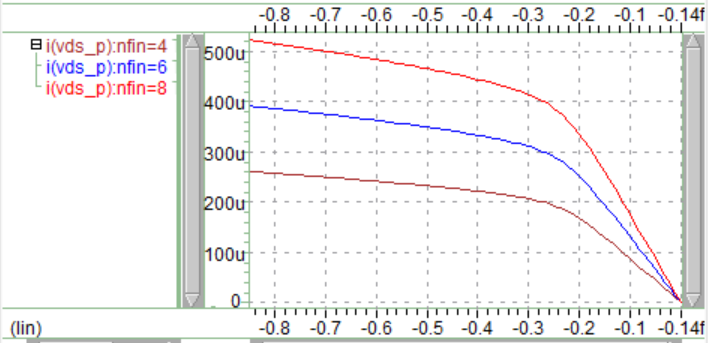
\includegraphics[width=\textwidth]{figure/wv_Task1_Fin_PFET.png} 
        \caption{PMOS: $I_{\text{DS}}-V_{\text{DS}}$}
        \label{fig:PFET_I_V}
    \end{subfigure}
    % 总图标题
    \caption{$I_{\text{DS}}-V_{\text{DS}}$ curve}
    \label{fig:FET_IV}
\end{figure}

\subsection{Task2. Measure important parameters}

\textbf{Requirements}

For both bulk silicon MOSFETs and FinFETs, for both N-Channel and P-Channel:
\begin{itemize}
	\item All metrics need to be measured at $25^\circ$C and $9^\circ$C respectively
	\item The supply voltage is 0.75V for both FinFETs and bulk Si-MOSFETs
	\item Width = 128nm for ptm16hp bulk Si-MOSFETs while fin number = 2 for ptm16hp FinFETs.
\end{itemize}


\textbf{Procedures}

\subsubsection{Measure $I_{\text{on}}$ and $I_{\text{off}}$}

For N-Channel, the on-state current $I_{\text{on}}$ is measured when $V_{\text{GS}}=V_{\text{DD}}$ and $V_{\text{DS}}=V_{\text{DD}}$ while the off-state current $I_{\text{off}}$ is measured when $V_{\text{GS}}=0$ and $V_{\text{DS}}=V_{\text{DD}}$.

For P-Channel, the on-state current $I_{\text{on}}$ is measured when $V_{\text{GS}}=0$ and $V_{\text{DS}}=-V_{\text{DD}}$ while the off-state current $I_{\text{off}}$ is measured when $V_{\text{GS}}=-V_{\text{DD}}$ and $V_{\text{DS}}=-V_{\text{DD}}$.

For bulk Silicon MOSFETs, the HSPICE codes to measure the two currents are as follows, which has considered situations both in $25^\circ$C and $90^\circ$C.
\begin{lstlisting}
    ************ temperature = 25 *****************
    .dc VG_N 0 0.8 0.01 
    .probe DC I(VG_N)
    .measure DC Ion_n FIND I(VD_N) WHEN V(gate_n) = 'supply'
    .measure DC Ioff_n FIND I(VD_N) WHEN V(gate_n) = 0
    .dc VG_P 0 -0.8 -0.01 
    .probe   DC I(VG_P)
    .measure DC Ion_p FIND I(VD_P) WHEN V(gate_p) = '-supply'
    .measure DC Ioff_p FIND I(VD_P) WHEN V(gate_p) = 0
    ************ temperature = 90 *****************
    .alter
    .temp 90
    .dc VG_N 0 0.8 0.01 
    .probe DC I(VG_N)
    .measure DC Ion_n FIND I(VD_N) WHEN V(gate_n) = 'supply'
    .measure DC Ioff_n FIND I(VD_N) WHEN V(gate_n) = 0
    .dc VG_P 0 -0.8 -0.01 
    .probe   DC I(VG_P)
    .measure DC Ion_p FIND I(VD_P) WHEN V(gate_p) = '-supply'
    .measure DC Ioff_p FIND I(VD_P) WHEN V(gate_p) = 0
\end{lstlisting}

When we consider FinFETs, the code is almost completely consistent, thus omitted here.

\subsubsection{Measure thershold voltage $V_{\text{T}}$}

Constant current method defines threshold as the gate voltage at a given drain current $I_{\text{crit}}$. A typical choice of $I_{\text{crit}}$ is $\frac{W}{L}\times 0.3\mu \text{A}$. In this experiment, we choose $\frac{W}{L}\times 0.3\mu \text{A}$ as $I_{\text{crit}}$. But it is worth noting that for different process, the width and length of the channel of the transistor are different. In bulk silicon MOSFETs, the length is 16nm and width is 128nm. However, in FinFETs, the length is 20nm and width is also 128nm, which is calculated by equation \eqref{eq:multiple_min} when the fin counts is 2.

Take the HSPICE code of measuring the $V_{\text{T}}$ of FinFETs as an example. In this time, we sweep the voltage of gate-source, from 0V to 0.8V for NFET and from 0V to -0.8V for PFET. What we should pay more attention to is that the level of source and bulk should be the same.
\begin{lstlisting}
    ************ temperature = 25 *****************
    .dc VG_N 0 0.8 0.01
    .probe DC I(VG_N)
    .measure DC VTH_n FIND V(gate_n) WHEN I(VD_N) = '-0.3u*Width/Lg_fin'
    .dc VG_P 0 -0.8 -0.01
    .probe DC I(VG_P)
    .measure DC VTH_p FIND V(gate_p) WHEN I(VD_P) = '0.3u*Width/Lg_fin'
    ************ temperature = 90 *****************
    .alter
    .temp 90
    .dc VG_N 0 0.8 0.01
    .probe DC I(VG_N)
    .measure DC VTH_n FIND V(gate_n) WHEN I(VD_N) = '-0.3u*Width/Lg_fin'
    .dc VG_P 0 -0.8 -0.01 
    .probe DC I(VG_P)
    .measure DC VTH_p FIND V(gate_p) WHEN I(VD_P) = '0.3u*Width/Lg_fin'
\end{lstlisting}


\textbf{Results}

\textbf{1. Widths/lengths of transistors} 

bulk Silicon MOSFETs: Length: 16nm, Width: 128nm

bulk Silicon MOSFETs: Length: 20nm, Width: 128nm

\textbf{2. Date Table} 

The turn-on current $I_{\text{on}}$, turn-off current $I_{\text{off}}$, and threshold voltage $V_{\text{T}}$ of MOSFETs of different processes and channel types at different temperatures measured using the HSPICE measure statement are shown in Tab.\ref{I_V_temp25} and Tab.\ref{I_V_temp90}.
\setlength{\arrayrulewidth}{0.9pt} % 线条粗一些,可按需调
\begin{table}[h]
    \centering
    % 如果过宽,可取消注释用 \resizebox 缩放
    \resizebox{\textwidth}{!}{%
    \begin{tabular}{|P{2.6cm}|P{2.6cm}|P{4.0cm}|P{2.2cm}|P{2.2cm}|P{2.4cm}|P{1.8cm}|}
        \hline
        % ----------------------- 表头 ------------------------
        \makecell{Process} & Channel & \makecell{Width/Width$_{\text{eff}}$(nm)} &
        $I_{\text{on}}$ & $I_{\text{off}}$ & $I_{\text{on}}/I_{\text{off}}$ & $V_{\text{T}}$ \\
        % ----------------------- 主体内容 ------------------------
        \cline{1-7}
        \multirow{2}{*}{Bulk}   & NMOS & 128 & 200.1$\mu$A & 85.42nA & 2343 & 0.1465V \\
        \cline{2-7}
                                & PMOS & 128 & 142.1$\mu$A & 116.5nA & 1220 & -0.1364V \\
        \cline{1-7}
        \multirow{2}{*}{FinFET} & NMOS & \makecell{128 (Fin num=2)} & 144.5$\mu$A & 9.412nA & 15353 & 0.1758V \\
        \cline{2-7}
                                & PMOS & \makecell{128 (Fin num=2)} & 126.9$\mu$A & 8.594nA & 14766 & -0.1800V \\
        \hline
    \end{tabular}}
    \caption{$I_{\text{on}}$, $I_{\text{off}}$ and $V_{\text{T}}$ for four transistors at temp = $25^\circ$C}
    \label{I_V_temp25}
\end{table}

\setlength{\arrayrulewidth}{0.9pt} % 线条粗一些,可按需调
\begin{table}[h]
    \centering
    % 如果过宽,可取消注释用 \resizebox 缩放
    \resizebox{\textwidth}{!}{%
    \begin{tabular}{|P{2.6cm}|P{2.6cm}|P{4.0cm}|P{2.2cm}|P{2.2cm}|P{2.4cm}|P{1.8cm}|}
        \hline
        % ----------------------- 表头 ------------------------
        \makecell{Process} & Channel & \makecell{Width/Width$_{\text{eff}}$(nm)} &
        $I_{\text{on}}$ & $I_{\text{off}}$ & $I_{\text{on}}/I_{\text{off}}$ & $V_{\text{T}}$ \\
        % ----------------------- 主体内容 ------------------------
        \cline{1-7}
        \multirow{2}{*}{Bulk}   & NMOS & 128 & 168.3$\mu$A & 185nA & 910 & 0.1377V \\
        \cline{2-7}
                                & PMOS & 128 & 92.59$\mu$A & 204.7nA & 452 & -0.1333V \\
        \cline{1-7}
        \multirow{2}{*}{FinFET} & NMOS & \makecell{128 (Fin num=2)} & 157.3$\mu$A & 89.76nA & 1752 & 0.1246V \\
        \cline{2-7}
                                & PMOS & \makecell{128 (Fin num=2)} & 141.4$\mu$A & 127.5nA & 1109 & -0.1120V \\
        \hline
    \end{tabular}}
    \caption{$I_{\text{on}}$, $I_{\text{off}}$ and $V_{\text{T}}$ for four transistors at temp = $90^\circ$C}
    \label{I_V_temp90}
\end{table}


\subsubsection{Measure Subthrehold Slope(SS)}

\textbf{Procedures}

The subthreshold slope is defined as the change in voltage for every tenfold change in current in the subthreshold region. Therefore, using the constant current method, given a current, simulation can determine the gate-source voltage of the transistor at that current and one-tenth of that current. The difference provides an approximate value for the subthreshold slope.

It is worth noting that as the aspect ratio increases, transistor drain-source current increases, and the selected constant current should also increase accordingly. Therefore, at the same temperature, since the aspect ratio of FinFETs is 6.4 and that of bulk Silicon MOSFETs is 8, the constant current selected for FinFETs should be smaller than that for bulk Silicon MOSFETs. Furthermore, as temperature increases, the transistor threshold voltage decreases, and the selected constant current should also increase accordingly.

Take the HSPICE code of measuring the $V_{\text{T}}$ of bulk Silicon as an example. In this time, we sweep the voltage of gate-source, from 0V to 0.8V for NMOS and from 0V to -0.8V for PMOS. When we find the current $I_{\text{DS}}$ reaching the specified value, we record the current gate voltage. The voltage difference between the two recordings is the subthreshold slope.

\textbf{results}

bulk Silicon MOSFETs: Length: 16nm, Width: 128nm

bulk Silicon MOSFETs: Length: 20nm, Width: 128nm

\textbf{2. Date Table} 

The SS of MOSFETs of different processes and channel types at different temperatures measured using the HSPICE measure statement are shown in Tab.\ref{SS_temp25} and Tab\ref{SS_temp90}.
\setlength{\arrayrulewidth}{0.9pt} % 线条粗一些,可按需调
\begin{table}[h]
    \centering
    % 如果过宽,可取消注释用 \resizebox 缩放
    \resizebox{\textwidth}{!}{%
    \begin{tabular}{|P{2.6cm}|P{2.6cm}|P{4.0cm}|P{2.2cm}|P{2.2cm}|P{2.4cm}|}
        \hline
        % ----------------------- 表头 ------------------------
        \makecell{Process} & Channel & \makecell{Width/Width$_{\text{eff}}$(nm)} &
        $V_1$ & $V_2$ & SS \\
        % ----------------------- 主体内容 ------------------------
        \cline{1-6}
        \multirow{2}{*}{Bulk}   & NMOS & 128 & 0.1727V & 0.06428V & 0.1084V/dec  \\
        \cline{2-6}
                                & PMOS & 128 & -0.1640V & -0.05218V & 0.1118V/dec  \\
        \cline{1-6}
        \multirow{2}{*}{FinFET} & NMOS & \makecell{128 (Fin num=2)} & 0.1875V & 0.1055V &  0.082V/dec \\
        \cline{2-6}
                                & PMOS & \makecell{128 (Fin num=2)} & -0.2017V & -0.1160V & 0.0917V/dec  \\
        \hline
    \end{tabular}}
    \caption{SS for four transistors at temp = $25^\circ$C}
    \label{SS_temp25}
\end{table}

\setlength{\arrayrulewidth}{0.9pt} % 线条粗一些,可按需调
\begin{table}[h]
    \centering
    % 如果过宽,可取消注释用 \resizebox 缩放
    \resizebox{\textwidth}{!}{%
    \begin{tabular}{|P{2.6cm}|P{2.6cm}|P{4.0cm}|P{2.2cm}|P{2.2cm}|P{2.4cm}|}
        \hline
        % ----------------------- 表头 ------------------------
        \makecell{Process} & Channel & \makecell{Width/Width$_{\text{eff}}$(nm)} &
        $V_1$ & $V_2$ & SS \\
        % ----------------------- 主体内容 ------------------------
        \cline{1-6}
        \multirow{2}{*}{Bulk}   & NMOS & 128 & 0.1802V & 0.04894V & 0.1331V/dec  \\
        \cline{2-6}
                                & PMOS & 128 & -0.1787V & -0.04347V & 0.1352V/dec  \\
        \cline{1-6}
        \multirow{2}{*}{FinFET} & NMOS & \makecell{128 (Fin num=2)} & 0.1381V & 0.04102V & 0.097V/dec  \\
        \cline{2-6}
                                & PMOS & \makecell{128 (Fin num=2)} & -0.1257V & -0.02725V &  0.0985V/dec \\
        \hline
    \end{tabular}}
    \caption{SS for four transistors at temp = $90^\circ$C}
    \label{SS_temp90}
\end{table}

\newpage
\section{Technical Analysis of the Simulation Results}
\subsection{Measurement methods}
In this lab, key device parameters are extracted using HSPICE measurement statements.

$I_{\text{on}}$ and $I_{\text{off}}$ are measured by fixing VGS and VDS at supply voltage levels corresponding to ON and OFF states, respectively. For NMOS, Ion is obtained at (VGS = VDD, VDS = VDD), while Ioff is taken at (VGS = 0, VDS = VDD). For PMOS, symmetric conditions with negative supply are applied.

Threshold voltage $V_{\text{T}}$ is extracted using the constant current method, with $I_{\text{crit}}=\frac{W}{L}\times 0.3\mu \text{A}$.

Subthreshold slope $\text{SS}$ is measured by identifying the gate voltages corresponding to drain currents differing by one decade (e.g., 0.5 $\mu$A and 0.05 $\mu$A for NMOS in $25^\circ$C), and calculating the voltage difference.

\subsection{Effect of Channel Width Variation on Device Characteristics}
Fig.\ref{fig:bulk_IV} shows that for both NMOS and PMOS transistors, when the gate length remains constant and the gate width increases from 128nm to 384nm in a planar silicon process, drain-source current increases nearly threefold across all voltage ranges. For example, at a drain voltage of 0.75V, the drain-source current is approximately 200$\mu$A with a 128nm gate width, but increases to 600$\mu$A with a 384nm gate width.

A similar phenomenon occurs in FinFET processes. When the number of fins increases from 4 to 8, the transistor's drain-source current also increases by a factor of two, as shown in Fig.\ref{fig:FET_IV}. This is because the gate width is proportional to the number of fins.

The nearly linear increase in on-state drain-source current with increasing aspect ratio can be reflected by the following drain-source current equation:
\begin{equation}
    I_{\text{DS}} = k'\frac{W}{L}[(V_{\text{GS}}-V_{\text{min}})V_{\text{min}}-\frac{1}{2}V_{\text{min}}^2], V_{\text{min}}=\min\{V_{\text{GT}}, V_{\text{DSAT}}, V_{\text{DS}}\}
    \label{leakage_equation}
\end{equation}

\subsection{Effects of Temperature Variation on Device Characteristics}
Temperature effects exhibited significant technology dependence. At $90^\circ$C compared to $25^\circ$C:

\textbf{For bulk silicon MOSFETs:} 
$I_{\text{on}}/I_{\text{off}}$ ratio decreased by 61\% for NMOS (2343 $\rightarrow$ 910) and 63\% for PMOS (1220 $\rightarrow$ 452), primarily due to $I_{\text{off}}$ increasing by 117\% for NMOS and 76\% for PMOS.

\textbf{FinFETs} 
$I_{\text{on}}/I_{\text{off}}$ ratio decreased by 89\% for NMOS (15353 $\rightarrow$ 1752) and 92\% for PMOS (14766 $\rightarrow$ 1109), with more rapid $I_{\text{off}}$ increases.

The threshold voltage temperature coefficient was more pronounced in FinFETs, with $V_T$ decreasing by 29\% for NFET and 38\% for PFET, compared to 6\% and 2\% respectively in bulk devices. This proves why the off-state current of FinFET increases so dramatically when the temperature increases from $25^\circ$C Celsius to $90^\circ$C Celsius. Because we have eq.\ref{eq:sub_current}:
\begin{equation}
    I_{\text{DS}_\text{sub}}\propto e^{\frac{V_{\text{GS}}-V_{\text{T}}}{nV_{\text{T}}}}
    \label{eq:sub_current}
\end{equation}

This suggests different carrier transport mechanisms and mobility temperature dependence between the two technologies.

\subsection{Comparison of different devices: bulk Si-MOSFETs and FinFET}
The data from Tab.\ref{I_V_temp25} and Tab.\ref{I_V_temp90} reveals FinFET's obvious advantages in nanoscale regimes:

\textbf{Leakage Performance:} FinFETs show dramatically lower off-state currents: 9.4nA vs 85.4nA for NMOS and 8.6nA vs 116.5nA for PMOS at $25^\circ$C, representing 89\% and 93\% reduction respectively. This severe deterioration can be seen in the Fig.\ref{fig:Ioff_comparison}. The blue curve represents the $I_{\text{DS}}-V_{\text{GS}}$ curve at $25^\circ$C, and the red curve represents the case at $90^\circ$C. It can be obviously seen that the leakage current at $90^\circ$C has increased significantly compared to the case at $25^\circ$C.
\begin{figure}[htbp]
    \center
    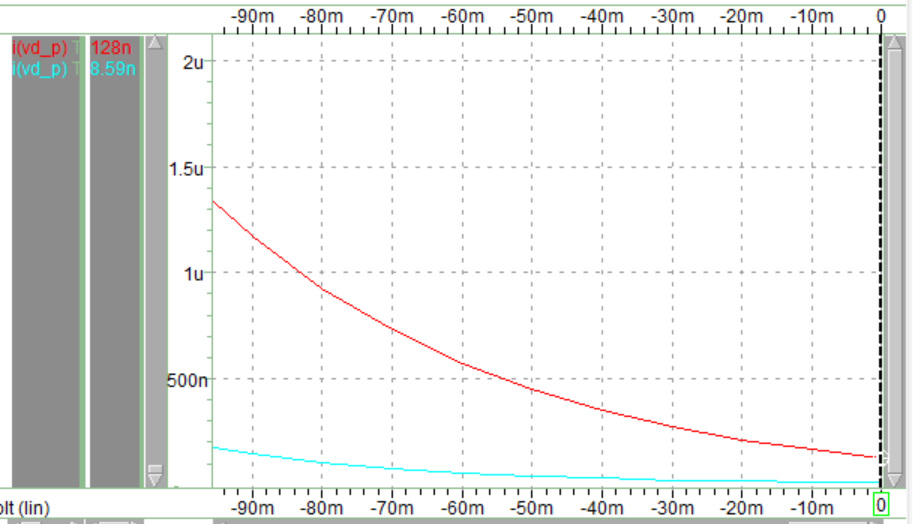
\includegraphics[width=0.8\textwidth]{figure/wv_FinFET_25_90_off.png}
    \caption{$I_{\text{off}}$ comparison for PFET at $25^\circ$C and $90^\circ$C}
    \label{fig:Ioff_comparison}
\end{figure}

\textbf{Current Ratio:} The $I_{\text{on}}/I_{\text{off}}$ ratio favors FinFETs by 6.5 times for NMOS and 12 times for PMOS at $25^\circ$C, highlighting better switching characteristics.

\textbf{Electrostatic Control:} FinFETs exhibit superior subthreshold characteristics with SS values of 82-98 mV/dec compared to 108-135 mV/dec for bulk MOSFETs. The 25\% better SS at $25^\circ$C demonstrates enhanced gate control.

\newpage
\section{Observations and conclusions}


From the simulation experiments, several key observations can be made:

\textbf{About Temperature dependence:}

Both bulk silicon MOSFETs and FinFETs experience an increase in off-state leakage current $I_{\text{off}}$ with rising temperature. However, the increase is much more pronounced in FinFETs. This is consistent with the stronger temperature sensitivity of FinFET threshold voltage, which drops significantly as temperature rises. The sharp reduction in $V_{\text{T}}$ shifts the device into stronger inversion even at low gate voltages, resulting in a dramatic Ioff increase.

\textbf{About Device comparison:}

At room temperature, FinFETs clearly outperform bulk MOSFETs with lower leakage current, higher $I_{\text{on}}/I_{\text{off}}$ ratio, and steeper subthreshold slope. But at elevated temperature, while FinFETs still maintain advantages, their Ioff increases faster than in bulk devices, narrowing the performance gap.

\textbf{About my understanding to DIC course:}

Through this experiment, I learned the fundamentals of transistor-level circuit simulation using HSpice. By comparing bulk silicon MOSFETs and FinFETs, I also intuitively experienced the detrimental effects of rising temperature on transistor leakage, as well as the FinFET's highly effective gate-controlled structure in suppressing leakage at room temperature.

This experiment deepened my understanding of transistor-level design metrics in basic digital integrated circuits, including aspect ratio, leakage current, and subthreshold characteristics. This will be beneficial for my future studies.
% 参考文献如不需要,将如下两行注释掉
% \bibliographystyle{plain}
% \bibliography{./template}  %bib文件名

\end{document}
